\documentclass[11pt]{article}

\usepackage[letterpaper,margin=0.76in]{geometry}
\usepackage[T1]{fontenc}
\usepackage[utf8]{inputenc}
\usepackage{lmodern}
\usepackage{microtype}
\usepackage{amsmath,amssymb,bm,mathtools}
\usepackage{booktabs,tabularx,array}
\usepackage{graphicx}
\usepackage{xcolor}
\usepackage{hyperref}
\usepackage{enumitem}
\usepackage{fancyhdr}
\usepackage{float}
\usepackage{caption}
\usepackage{tikz}
\usetikzlibrary{arrows.meta,positioning}

\definecolor{deepblue}{RGB}{29,68,112}
\definecolor{softblue}{RGB}{235,242,249}
\definecolor{softgray}{RGB}{245,246,247}
\definecolor{darkgray}{RGB}{70,70,70}

\hypersetup{
  colorlinks=true,
  linkcolor=deepblue,
  citecolor=deepblue,
  urlcolor=deepblue,
  pdftitle={First-Principles Coherent and Surface-Hopping Charge-Transfer Dynamics in 2H2Pc/C60},
  pdfauthor={Amirhosein Amini}
}

\pagestyle{fancy}
\fancyhf{}
\lhead{$2\mathrm{H_2Pc}/\mathrm{C}_{60}$ charge-transfer dynamics}
\rhead{CyberTraining 2026 Capstone}
\cfoot{\thepage}
\setlength{\headheight}{14pt}

\setlength{\parindent}{0pt}
\setlength{\parskip}{0.42em}
\setlist[itemize]{leftmargin=1.5em,itemsep=0.12em,topsep=0.2em}
\setlist[enumerate]{leftmargin=1.7em,itemsep=0.18em,topsep=0.25em}
\captionsetup{font=small,labelfont=bf}

\newcommand{\Csixty}{\mathrm{C}_{60}}
\newcommand{\HtwoPc}{\mathrm{H_2Pc}}
\newcommand{\code}[1]{\texttt{#1}}
\newcommand{\highlight}[1]{%
  \begin{center}
  \fcolorbox{deepblue}{softblue}{\parbox{0.92\textwidth}{#1}}
  \end{center}}

\title{\vspace{-1.4em}\textbf{First-Principles Coherent and Surface-Hopping\\Charge-Transfer Dynamics in $2\HtwoPc/\Csixty$}\\[0.35em]
\large A PySCF--Libra Study with a Validated Reduced Hamiltonian}
\author{Amirhosein (Amir) Amini\\
Department of Chemistry, Texas A\&M University\\
Advisor: Prof. Arkajit Mandal}
\date{July 17, 2026}

\begin{document}
\maketitle
\vspace{-1.15em}

\begin{abstract}
In this work, we develop a first-principles workflow for early-time charge-transfer dynamics in the 176-atom $2\HtwoPc/\Csixty$ donor--acceptor complex introduced by Yamijala and Huo. We replace the DFTB3 Hamiltonian used in the reference work with a PySCF-derived Kohn--Sham Hamiltonian sampled along ten independent 100 fs molecular-dynamics trajectories. The active orbitals are tracked using cross-geometry overlaps, optimal assignment, a closest-unitary polar factor, and matrix-logarithm orbital derivative couplings. We propagate the resulting ten-state Hamiltonians using exact matrix exponentials and Libra classical-path fewest-switches surface hopping. We then construct an independently propagated four-donor plus three-acceptor model and evaluate pair-resolved probability currents. We find that the reduced model reproduces the full coherent ensemble with an RMSE of 0.0183. Plain CPA-FSSH underestimates the digitized experimental transfer, whereas Boltzmann-rescaled upward hops overestimate it. The pathway analysis reveals strong donor--acceptor coherence and substantial recrossing: the most dynamically active pair is not the largest source of net acceptor accumulation. Overall, the results show that the predicted transfer kinetics are strongly sensitive to the electronic Hamiltonian and detailed-balance prescription, while the state tracking and reduced-model construction are numerically robust. This capstone is exclusively a theoretical charge-transport study and contains no cybersecurity or biological component.
\end{abstract}

\section{Motivation and scientific question}
Photoinduced charge transfer in donor--acceptor complexes is often reduced to one donor state, one acceptor state, and a single coupling. That picture is inadequate for $2\HtwoPc/\Csixty$. The phthalocyanine and fullerene manifolds contain several nearly degenerate orbitals, nuclear motion continuously rotates these orbitals, and the experimentally relevant observable is a fragment charge rather than the population of one adiabatic state.

\highlight{\textbf{How do coherent electronic dynamics, stochastic surface hopping, detailed balance, and active-space reduction control the predicted early-time $\Csixty$ charge population?}}

The goal is not to tune the calculation to the published curve. Instead, each transformation from the molecular geometry to the final fragment population is explicitly defined and independently tested.

\section{System and computational workflow}
The neutral complex has formula $\mathrm{C}_{124}\mathrm{H}_{36}\mathrm{N}_{16}$, 176 atoms, and 892 electrons. Atoms 1--116 form the two-phthalocyanine donor and atoms 117--176 form the fullerene acceptor.

\begin{figure}[H]
\centering
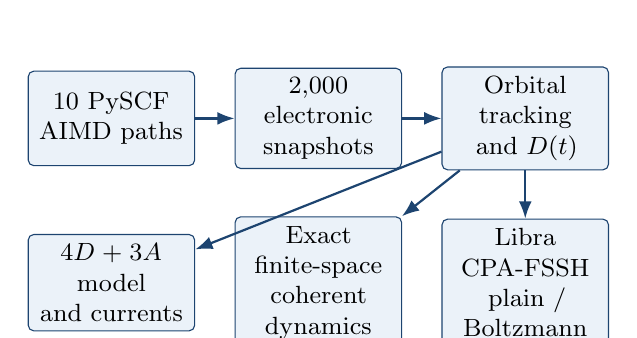
\begin{tikzpicture}[
  node distance=6mm and 5mm,
  box/.style={draw=deepblue,rounded corners=2pt,fill=softblue,
    align=center,text width=0.155\textwidth,minimum height=12mm,
    font=\small},
  arrow/.style={-{Latex[length=2.2mm]},thick,draw=deepblue}
]
\node[box] (aimd) {10 PySCF\\AIMD paths};
\node[box,right=of aimd] (snap) {2,000 electronic\\snapshots};
\node[box,right=of snap] (track) {Orbital tracking\\and $D(t)$};
\node[box,below=of snap] (coh) {Exact finite-space\\coherent dynamics};
\node[box,right=of coh] (libra) {Libra CPA-FSSH\\plain / Boltzmann};
\node[box,left=of coh] (reduce) {$4D+3A$ model\\and currents};
\draw[arrow] (aimd) -- (snap);
\draw[arrow] (snap) -- (track);
\draw[arrow] (track) -- (coh);
\draw[arrow] (track) -- (libra);
\draw[arrow] (track) -- (reduce);
\end{tikzpicture}
\caption{Computational workflow used in this work. Every retained branch produces a directly testable observable or numerical diagnostic.}
\end{figure}

The calculation consists of six steps:
\begin{enumerate}
\item generate ten independent 100 fs, 300 K nuclear paths with PySCF Born--Oppenheimer AIMD;
\item compute ten low-lying virtual Kohn--Sham orbitals and a $\Csixty$ fragment projector at every 0.5 fs frame;
\item track the active space and construct orbital time-derivative couplings;
\item propagate the full ten-state Hamiltonian coherently and with Libra CPA-FSSH;
\item construct and validate a fragment-adapted $4D+3A$ Hamiltonian;
\item resolve the coherent transfer into donor-to-acceptor probability-current channels.
\end{enumerate}

\section{Methods}
\subsection{Electronic structure, active space, and state tracking}
We propagate the nuclei using PBE-D3(BJ)/6-31G, density fitting, and a 0.5 fs nuclear time step. The trajectories are ground-state, thermostatted paths and therefore provide a prescribed fluctuating environment rather than electronically back-reacted nonadiabatic nuclear dynamics.

At each geometry, the active space consists of the first ten unoccupied Kohn--Sham orbitals. The initial electronic state is obtained by projecting the isolated donor-dimer LUMO into this space,
\begin{equation}
 b_i=\langle\psi_i|\phi_D\rangle,
 \qquad
 c_i(0)=\frac{b_i}{\sqrt{\sum_j|b_j|^2}}.
\end{equation}

For adjacent geometries, we form the cross-geometry overlap
\begin{equation}
 O_{ij}^{(n)}=\left\langle\psi_i(\bm R_n)\middle|\psi_j(\bm R_{n+1})\right\rangle.
\end{equation}
A Hungarian assignment maximizes the total absolute overlap, and matched orbital signs are chosen to make the diagonal overlaps positive. If $\bm O=\bm L\bm\Sigma\bm R^\dagger$, the closest-unitary polar factor is $\bm U=\bm L\bm R^\dagger$. The midpoint orbital derivative-coupling matrix and propagated vibronic Hamiltonian are
\begin{equation}
 \bm D_{n+1/2}=\frac{1}{\Delta t}\log\bm U_n,
 \qquad
 \bm H_{\mathrm{vib},n+1/2}=\bm E_{n+1/2}-i\bm D_{n+1/2}.
\end{equation}
These are Kohn--Sham orbital time-derivative couplings; no TDDFT excited-state calculation is performed.

\subsection{Coherent dynamics, fragment charge, and FSSH}
For each piecewise-constant midpoint Hamiltonian, the electronic amplitudes are propagated using
\begin{equation}
 \bm c(t+\Delta t)=\exp[-i\bm H_{\mathrm{vib}}\Delta t]\bm c(t).
\end{equation}
This propagation is numerically exact within the finite ten-state Hamiltonian. The coherent fullerene population is
\begin{equation}
 P_{\Csixty}(t)=\bm c^\dagger(t)\bm P_{\Csixty}(t)\bm c(t),
\end{equation}
where $\bm P_{\Csixty}$ is a symmetrized Mulliken fragment projector.

Libra evaluates active-state-specific fewest-switches probabilities for 20,000 stochastic surface histories on each nuclear path. In addition to plain CPA-FSSH, we evaluate a sensitivity model in which thermally uphill hops are multiplied by
\begin{equation}
 \exp\left[-\frac{E_j-E_i}{k_{\mathrm B}T}\right],\qquad E_j>E_i.
\end{equation}
The coherent amplitudes are unchanged between these two calculations; only the stochastic active-surface histories differ.

\subsection{Reduced Hamiltonian and pathway-resolved currents}
The reduced model contains the complete four-state donor subspace and the three lowest fullerene states. Both fragment subspaces are parallel transported between frames, and the seven-state Hamiltonian is constructed independently using the same polar-decomposition and matrix-logarithm procedure.

For donor state $d$ and acceptor state $a$, the instantaneous probability current is
\begin{equation}
 J_{d\rightarrow a}(t)=2\,\mathrm{Im}\left[H_{ad}(t)c_d(t)c_a^*(t)\right].
\end{equation}
The signed time integral measures net transfer. The positive integral measures total forward activity, while the absolute integral measures the full bidirectional exchange. These quantities distinguish a channel that accumulates acceptor population from one dominated by rapid recrossing.

\section{Results and interpretation}
\subsection{Tracking and reduced-model validation}
Across all 2,000 snapshots, the minimum singular value of the consecutive ten-state overlap matrices is 0.999580. The active subspace therefore remains continuous even when near-degenerate fullerene orbitals rotate strongly within their manifold.

At 99.5 fs, the full ten-state coherent ensemble gives
\begin{equation}
 P_{\Csixty}^{10\mathrm{s}}=0.2798\pm0.0963,
\end{equation}
while the independently constructed $4D+3A$ model gives
\begin{equation}
 P_{\Csixty}^{4D+3A}=0.2462\pm0.0882.
\end{equation}
The uncertainties are 95\% confidence intervals across ten independent nuclear trajectories. The ensemble-curve RMSE is 0.018301, the mean trajectory-level RMSE is 0.025094, and the maximum difference between the fragment-projector and simple acceptor-subspace populations is 0.006402. These results establish that the seven-state Hamiltonian preserves the observable of interest over the full simulated interval.

\begin{figure}[H]
\centering
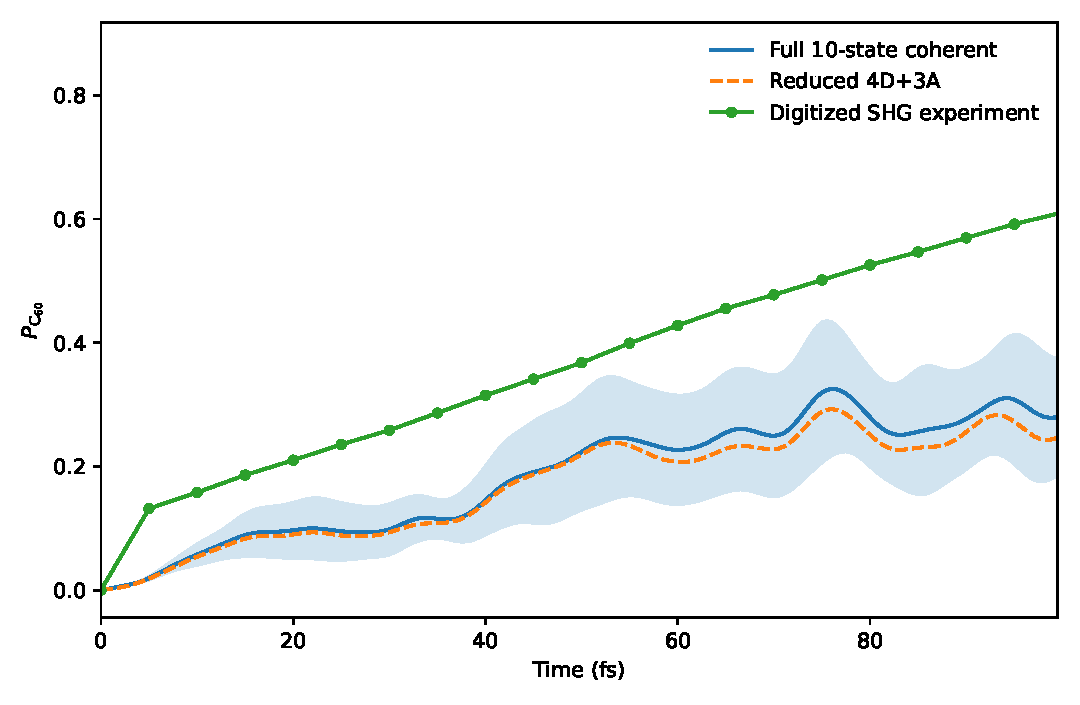
\includegraphics[width=0.94\textwidth]{../results/figures/coherent/coherent_full_vs_reduced.pdf}
\caption{Full ten-state coherent propagation, the independently constructed $4D+3A$ propagation, and the approximate digitized SHG experiment. The shaded region is the 95\% confidence interval of the full coherent ensemble across ten nuclear paths. The reduced curve follows the full active-space result throughout the simulated interval.}
\label{fig:coherent-reduction}
\end{figure}

\subsection{Surface-hopping sensitivity}
The approximate digitized experimental endpoint is 0.608567. Plain CPA-FSSH gives 0.280850 with a full-window RMSE of 0.192214. Boltzmann-rescaled FSSH gives 0.898903 with an RMSE of 0.304553.

\begin{figure}[H]
\centering
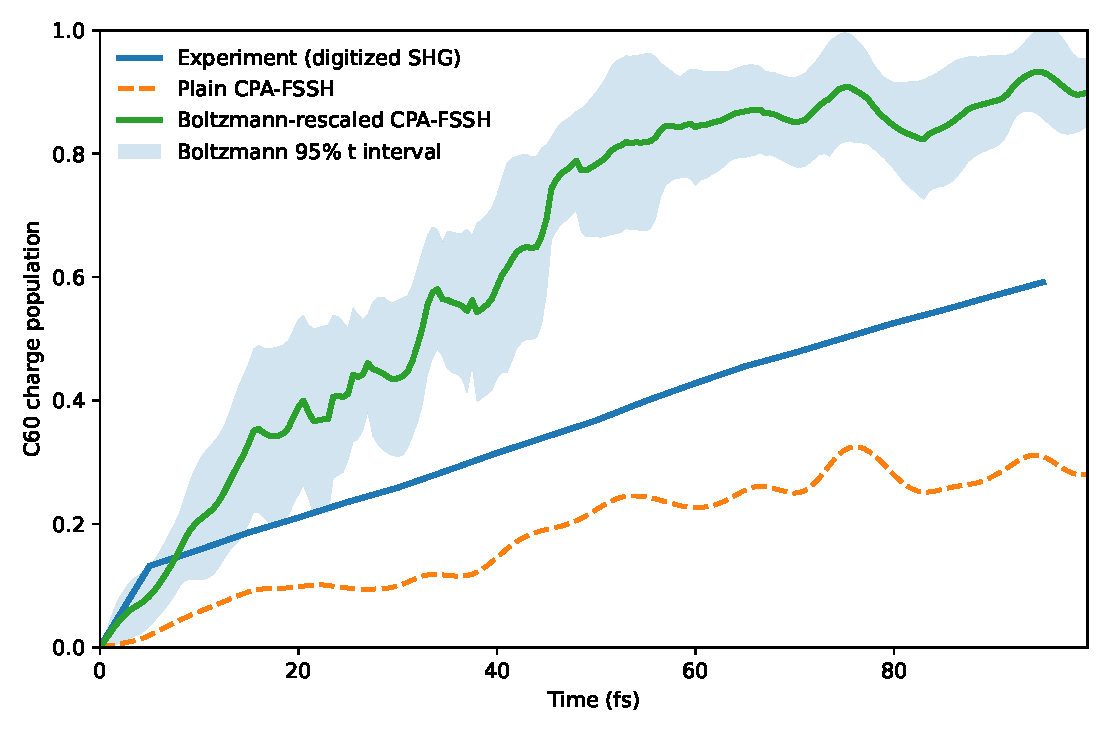
\includegraphics[width=0.94\textwidth]{../results/figures/libra/fig_plain_boltzmann_experiment.pdf}
\caption{Original Libra output comparing the digitized SHG experiment with the plain and Boltzmann-rescaled CPA-FSSH ensembles. The shaded band is the 95\% confidence interval for the Boltzmann-rescaled ensemble across ten nuclear trajectories. No empirical rescaling is applied to any curve.}
\label{fig:fssh-sensitivity}
\end{figure}

\highlight{\textbf{Interpretation.} Plain FSSH permits substantial uphill return and underestimates the observed transfer. Boltzmann rescaling strongly suppresses return from low fullerene states and overestimates the transfer. The experimental curve lies between the two predictions, demonstrating that detailed balance is a dominant physical-model choice rather than a universal correction.}

\subsection{Coherence, recrossing, and dominant pathways}
The maximum mean donor--acceptor coherence is 0.426162 at 77.5 fs, showing that the transfer cannot be represented as a sequence of completely incoherent one-way hops.

\begin{figure}[H]
\centering
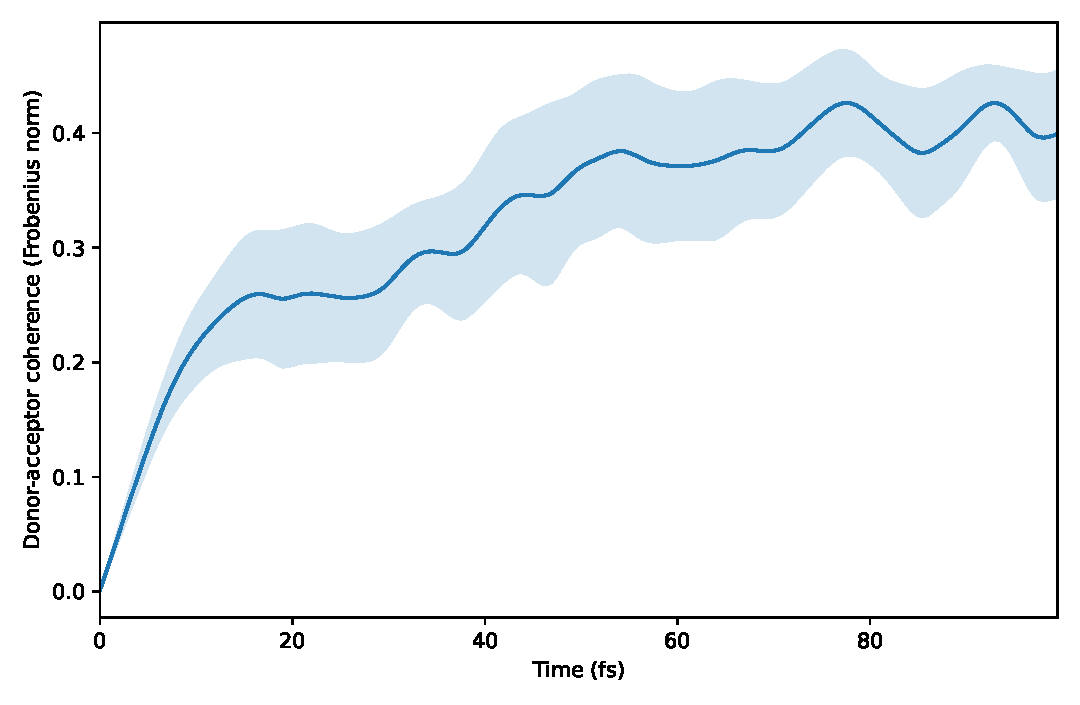
\includegraphics[width=0.94\textwidth]{../results/figures/coherent/donor_acceptor_coherence.pdf}
\caption{Mean donor--acceptor coherence, quantified by the Frobenius norm of the donor--acceptor density-matrix block. The shaded region is the 95\% confidence interval across ten nuclear trajectories.}
\label{fig:coherence}
\end{figure}

The most active forward channel is $D_2\rightarrow A_1$, with integrated positive flux 0.273903. However, its net signed flux is only 0.029675, whereas its absolute flux is 0.518130. Thus, $D_2\rightarrow A_1$ is the largest exchange channel but not the largest source of net acceptor accumulation.

\begin{figure}[H]
\centering
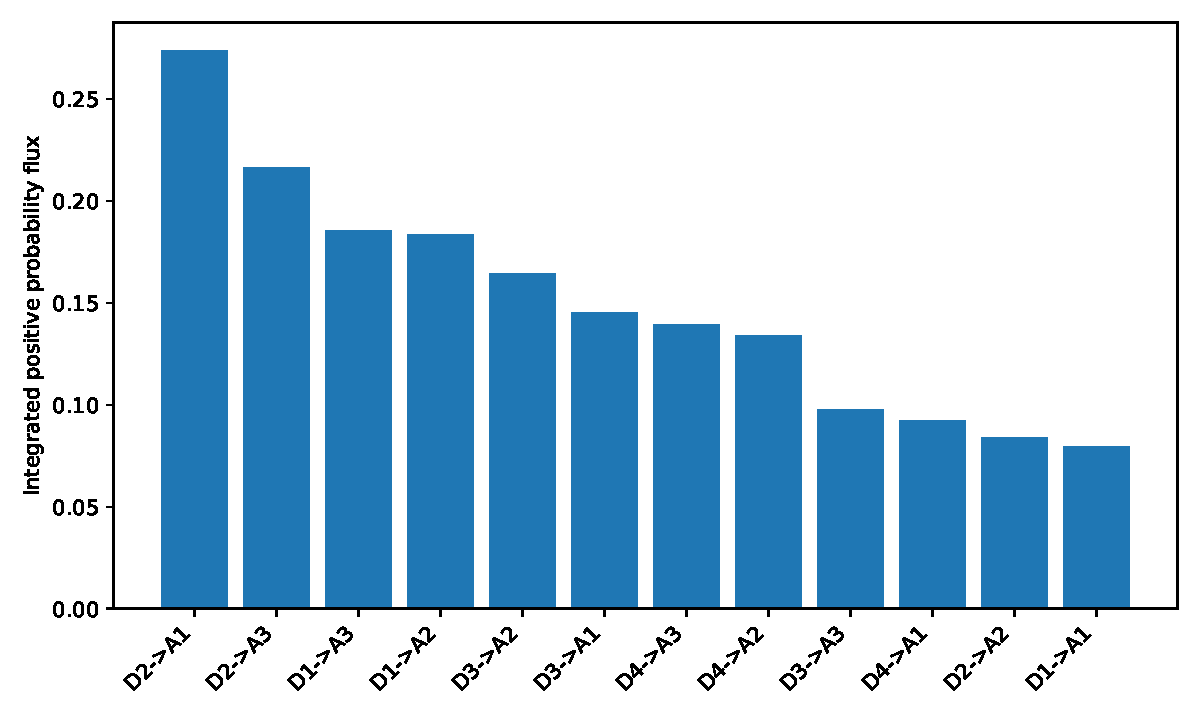
\includegraphics[width=0.96\textwidth]{../results/figures/coherent/dominant_transfer_channels.pdf}
\caption{Original pathway-analysis output showing the integrated positive probability flux for all twelve donor--acceptor pairs. $D_2\rightarrow A_1$ is the most dynamically active channel, but its signed integral is much smaller because the pair undergoes substantial recrossing.}
\label{fig:channels}
\end{figure}

The largest net-forward channels are $D_1\rightarrow A_3$ (0.072861), $D_1\rightarrow A_2$ (0.053819), $D_3\rightarrow A_2$ (0.049790), and $D_2\rightarrow A_3$ (0.041704). In contrast, $D_2\rightarrow A_2$ has a signed integral of $-0.036544$, indicating net backflow. Summing all twelve channel currents reproduces the time derivative of the acceptor population with a mean RMSE of $6.25\times10^{-5}$ fs$^{-1}$.

The complete signed, positive, and absolute pair currents are reported in \path{results/donor_acceptor_channel_flux.csv}; the time-resolved net current is retained as a supplementary output figure.

\section{Limitations and reproducibility}
The principal approximations are:
\begin{itemize}
\item ground-state Kohn--Sham orbitals replace many-electron excited states;
\item the nuclei follow prescribed, thermostatted paths with no electronic back-reaction;
\item no explicit decoherence correction is applied to the coherent amplitudes;
\item the experiment is digitized from a published figure and lacks original error bars;
\item exactness claims are restricted to propagation within the specified finite active-space Hamiltonian.
\end{itemize}

The source code, exact starting structures, random-seed protocol, portable Slurm launchers, compact outputs, figures, and report are available at
\begin{center}
\href{https://github.com/amiraminitamu/Summer-School-Buffalo}{\code{github.com/amiraminitamu/Summer-School-Buffalo}}.
\end{center}
Raw trajectories and frame-level arrays are excluded because of their multi-gigabyte size, but the retained inputs and scripts specify the complete regeneration path.

\section{Conclusions}
In this work, we develop a reproducible PySCF--Libra workflow that connects first-principles molecular trajectories, orbital tracking, finite-space coherent propagation, surface hopping, active-space reduction, and pathway-resolved probability currents for a 176-atom donor--acceptor complex.

We find that the $4D+3A$ Hamiltonian reproduces the full ten-state coherent ensemble with low error, establishing a compact mechanistic model. Charge transfer is multichannel and strongly recrossing: the most active donor--acceptor pair is not the largest contributor to net population accumulation. Plain CPA-FSSH underestimates the experimental transfer, whereas Boltzmann-rescaled upward hops overestimate it. Therefore, the remaining disagreement with experiment is controlled by the physical approximations in the electronic Hamiltonian, prescribed nuclear paths, and detailed-balance treatment, rather than by numerical instability in state tracking or propagation.

\section*{References}
\small
\begin{enumerate}[label={\arabic*.},leftmargin=1.6em]
\item S. R. K. C. Yamijala and P. Huo, ``Direct Nonadiabatic Simulations of the Photoinduced Charge Transfer Dynamics,'' \emph{J. Phys. Chem. A} \textbf{125}, 628--635 (2021), DOI: \href{https://doi.org/10.1021/acs.jpca.0c10151}{10.1021/acs.jpca.0c10151}.
\item Q. Sun \emph{et al.}, ``PySCF: the Python-based simulations of chemistry framework,'' \emph{WIREs Comput. Mol. Sci.} \textbf{8}, e1340 (2018).
\item A. V. Akimov, ``Libra: An open-source methodology-discovery library for quantum and classical dynamics simulations,'' \emph{J. Comput. Chem.} \textbf{37}, 1626--1649 (2016).
\item J. C. Tully, ``Molecular dynamics with electronic transitions,'' \emph{J. Chem. Phys.} \textbf{93}, 1061--1071 (1990).
\end{enumerate}

\end{document}
